\chapter{Dostupné datasety}
\label{sec:Datasets}
Před použitím konvoluční neuronové neuronové sítě navržené v této práci je nutné, aby byly váhy jednotlivých konvolucí správně nastaveny.
K tomuto účelu slouží tzv. trénovací množina.
Jedná se o množinu příkladů situací, na které může neuronová síť při svém fungování narazit.
V tomto případě, jelikož cílem sítě je určit počet lidí ve videosekvenci, se jedná o obrazy, resp. sekvenci po sobě jdoucích snímků.
Kromě samotných snímků potřebuje ještě síť základní pravdu, což je informace, pomocí které dokáže určit, jak moc se při svých predikcích mýlí, aby na základě této chyby mohla přenastavit své váhy, čímž tuto chybu sníží a posune se blíže optimu.
Tento typ strojového učení, kdy je pro natrénování modelu použita oanotovaná trénovací sada, se nazývá učení s učitelem.

Jelikož při samotném používání neuronové sítě již nedochází k žádnému přenastavování jejích vah, je pro zajištění jejího dobrého fungování naprosto stěžejní, aby byla trénovací množina rozsáhlá a co nejvíce různorodá.
Pokud je například síť natrénovaná pouze na snímcích získaných během dne, tak není zaručeno, že síť bude dosahovat stejně dobrých výsledků i na nočních záběrech.
Stejně tak model, natrénovaný na záběrech z bezpečnostních kamer, které jsou většinou umístěny vysoko nad lidskými hlavami, může mít problémy se záběry lidí pořízenými kamerou ve výšce očí.

Jelikož počítání lidí v obraze je mezi výzkumníky celkem populární problém, existuje k němu celá řada obsáhlých datasetů, z nichž některé jsou blíže popsány v této kapitole.
Mezi jednotlivými datasety ale mohou být veliké rozdíly a to nejen v rozlišení obsažených snímků, nebo velikosti davů, které snímky obsahují.
Rozdíly mohou být i v tom, jak jsou jednotlivé snímky anotovány, nebo v technologiích použítých pro pořízení těchto snímků.
To může být způsobeno například tím, kde má být daný estimátor nasazen, což bude určovat, jaké typy snímků bude dataset obsahovat.
Například datasety VisDrone \cite{VisDrone-Dataset-1, VisDrone-Dataset-2}, slouží k učení detekce, sledování a počítání objektů a lidí v obrazech a videích pořízených z dronu letícího desítky metrů nad zemí.
Oproti tomu snímky datasetu ShanghaiTechRGBD \cite{ShanghaiTechRGBD-1, ShanghaiTechRGBD-2} byly pořízeny ve zhruba dvoumetrové výšce pomocí RGB-D senzoru, což znamená, že kromě barevné složky snímky obsahují i hloubkovou informaci říkající, jak daleko od kamery se jednotlivé objekty ve scéně nacházejí.

\section{UCF-QNRF}
\begin{figure}[h!]
	\centering
	\subfloat[]{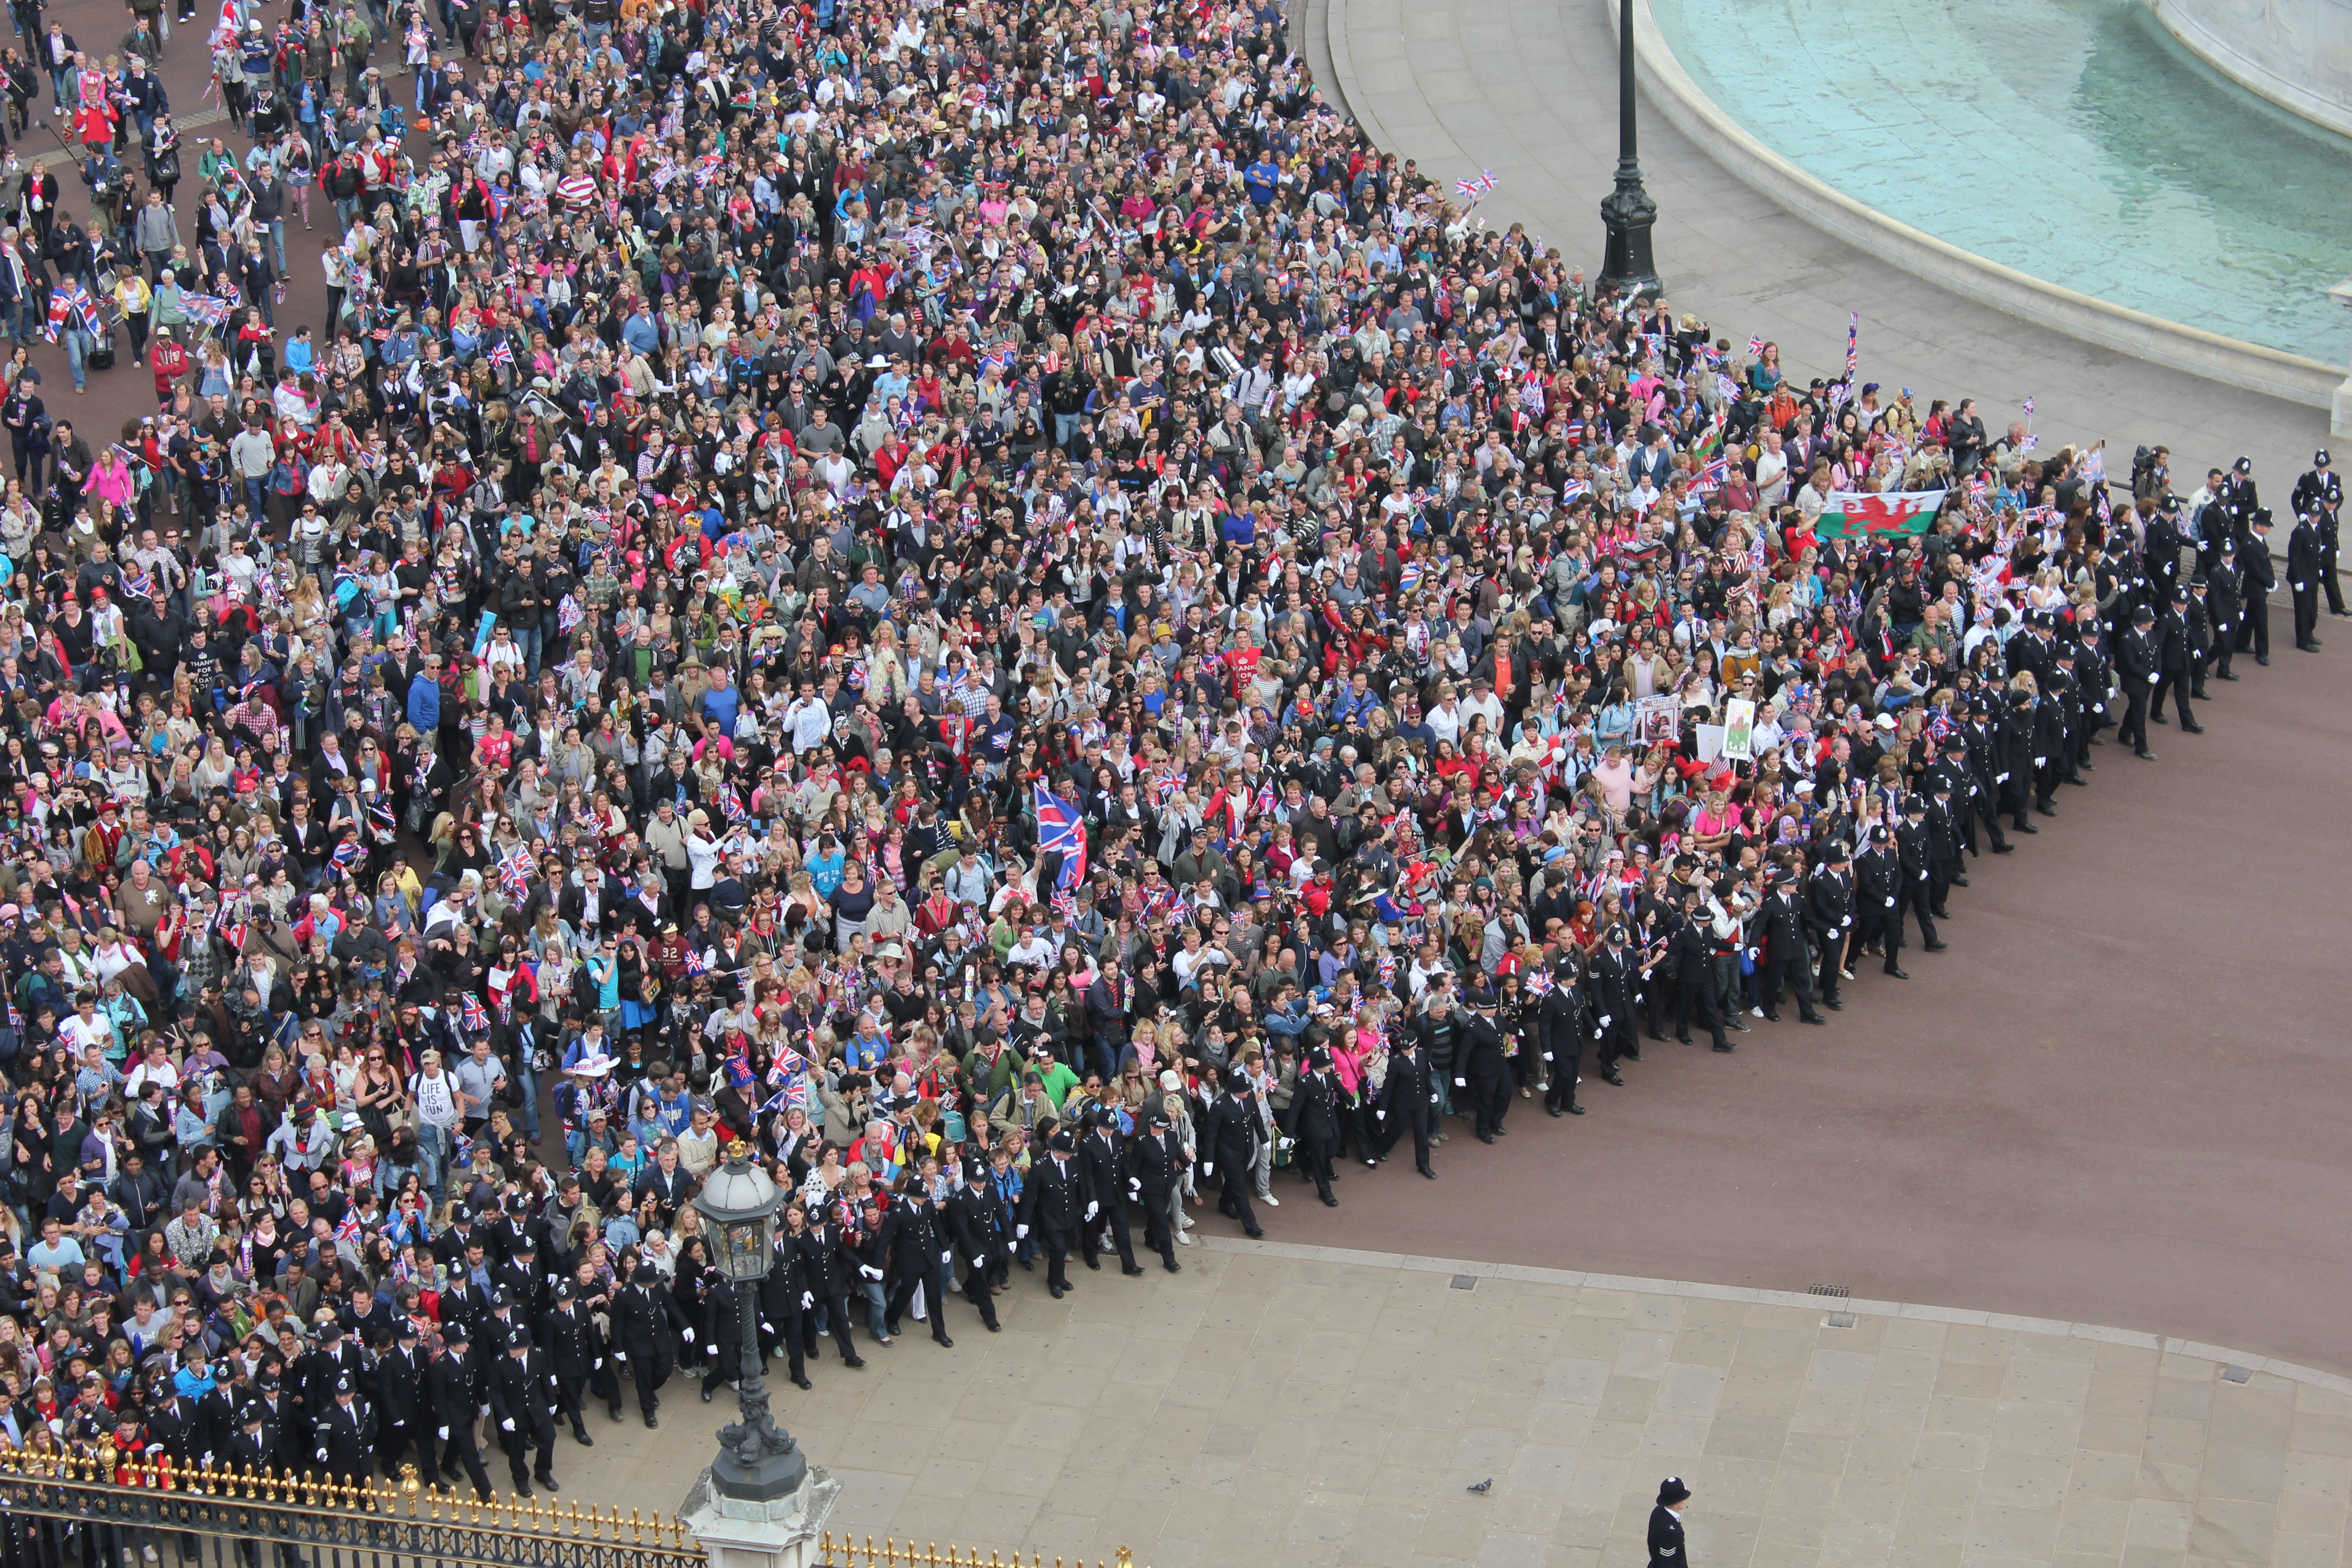
\includegraphics[height=3.5cm]{Figures/datasets/UCF-QNRF/img_0184.jpg}}
	\subfloat[]{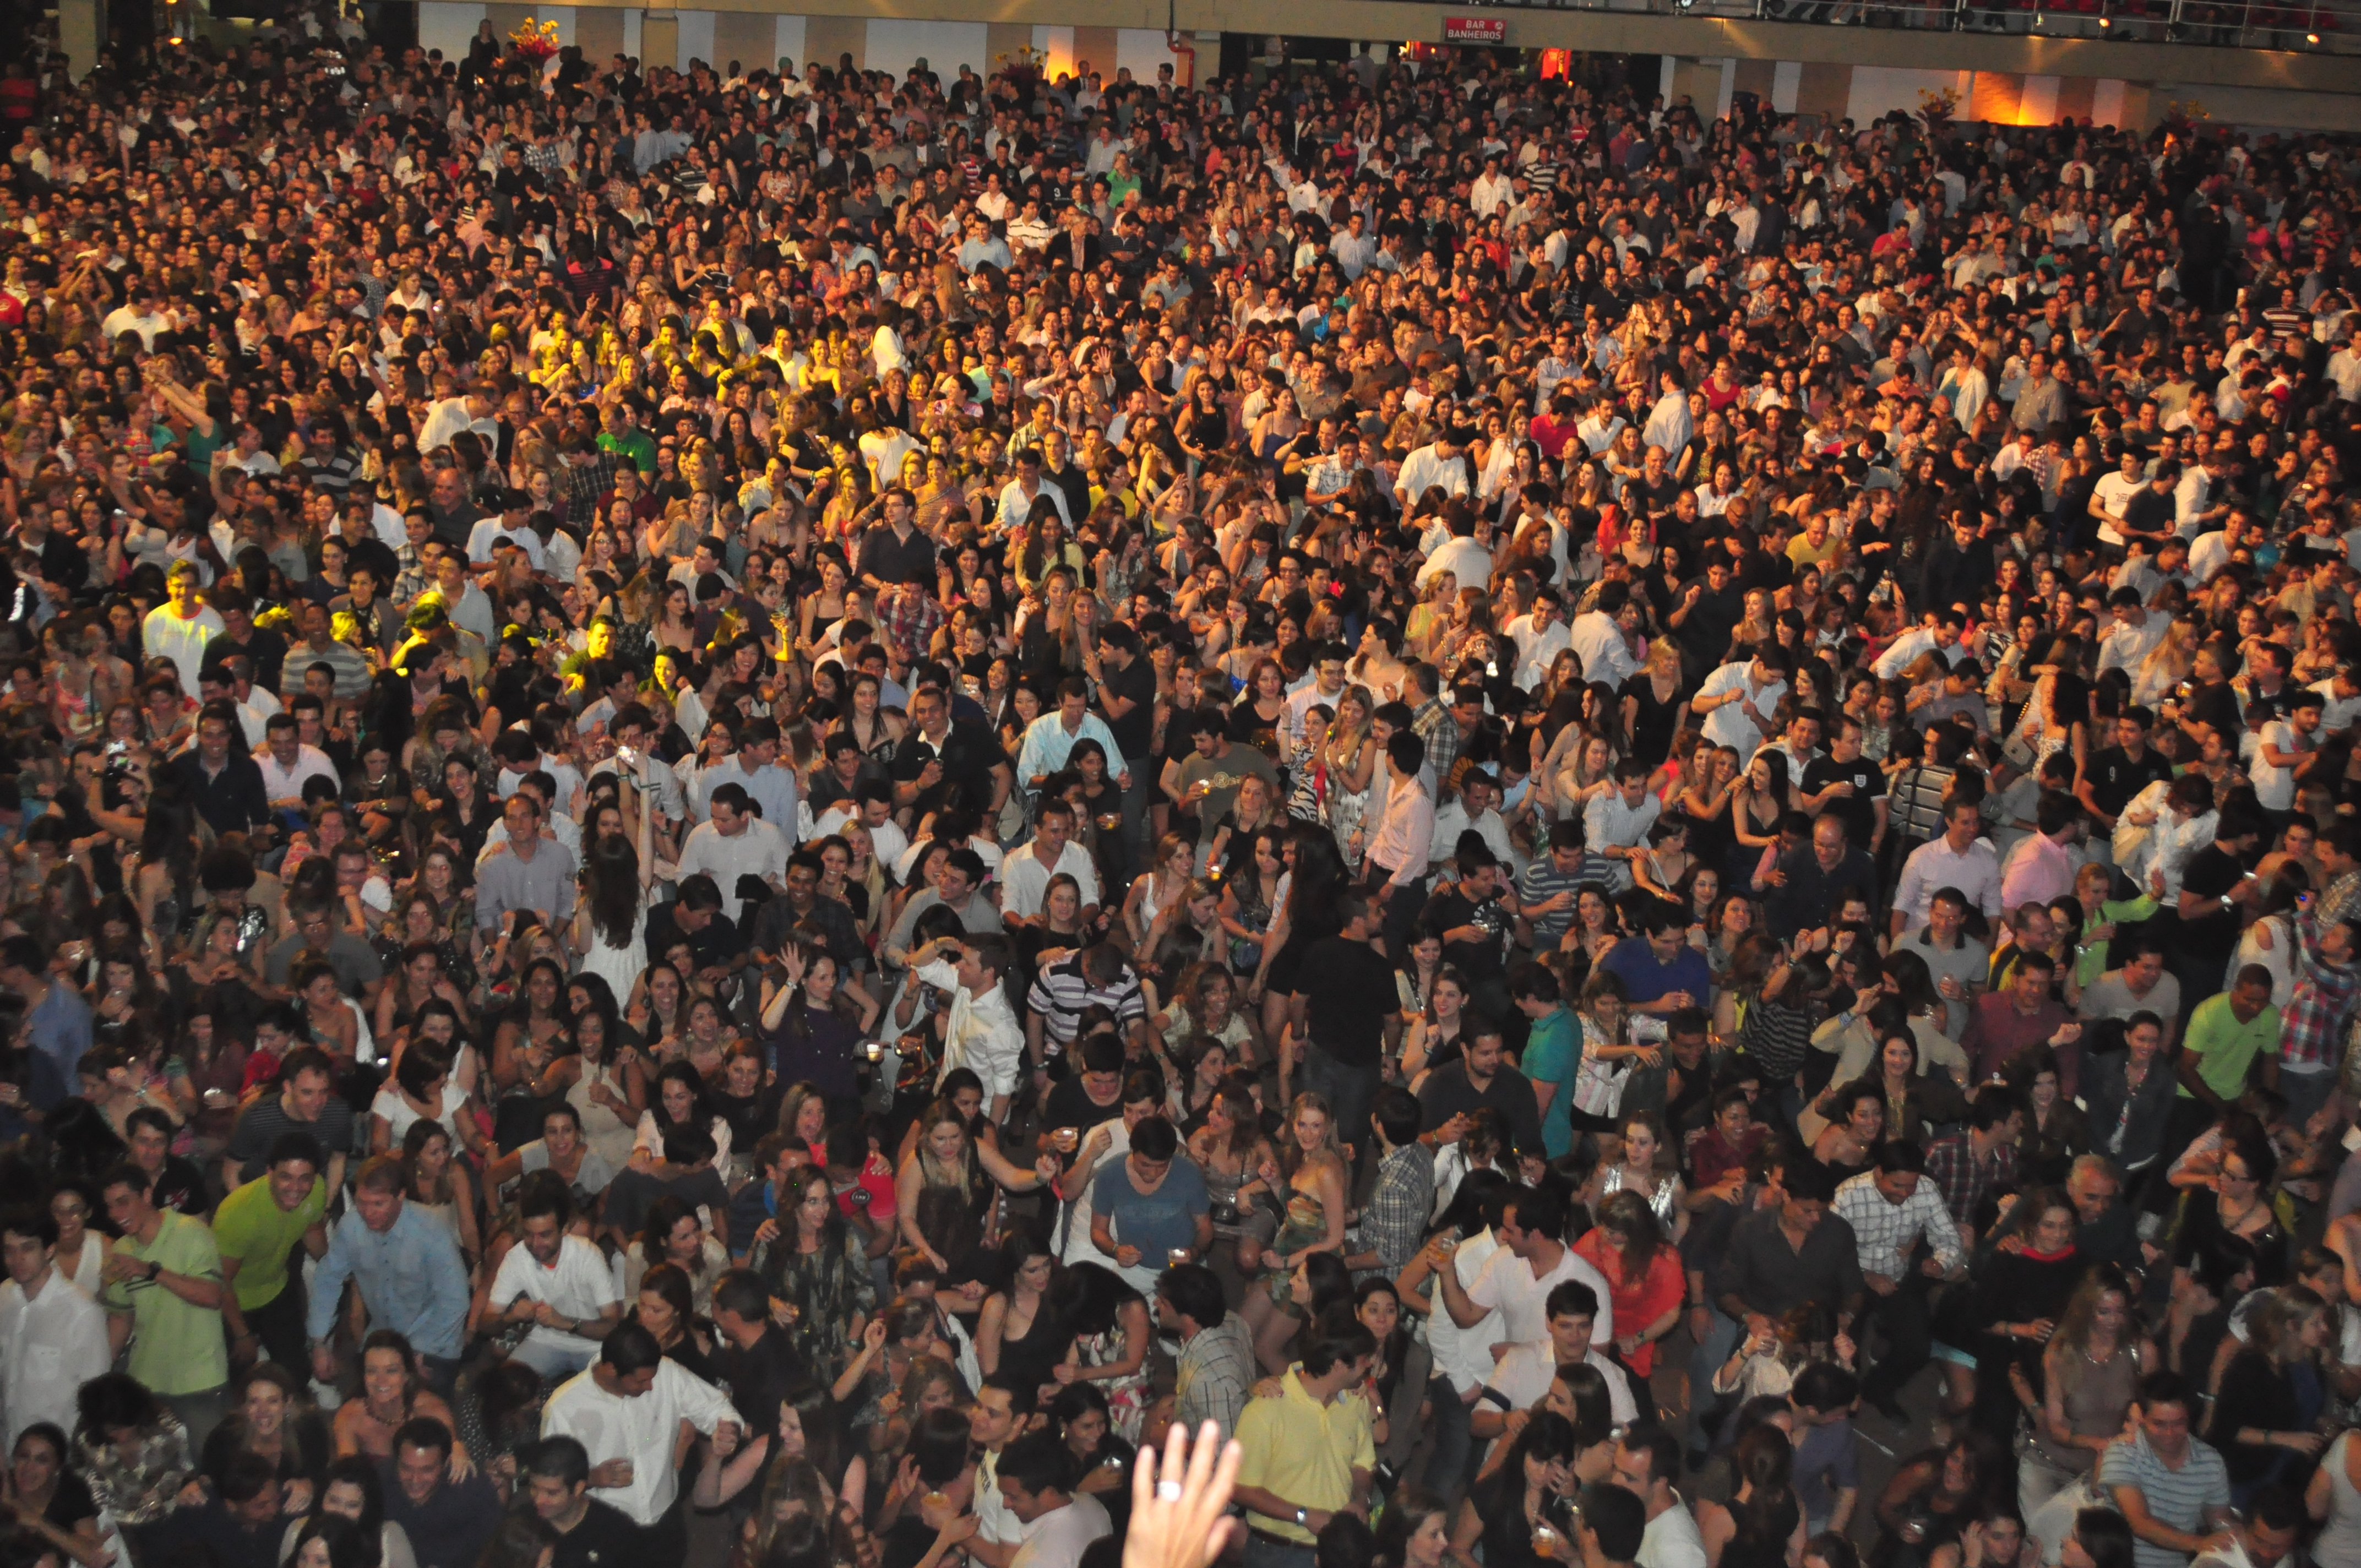
\includegraphics[height=3.5cm]{Figures/datasets/UCF-QNRF/img_0222.jpg}}
	\subfloat[]{\includegraphics[height=3.5cm]{Figures/datasets/UCF-QNRF/img_0330.jpg}}
	\caption{Ukázka snímků obsažených v datasetu UCF-QNRF \cite{QNRF}}
	\label{fig:QNRF}
\end{figure}

Dataset QNRF \cite{QNRF} z Univerzity střední Floridy (University of Central Florida) je jedním z nejpopulárnějších datasetů používaných pro trénování a validaci metod strojového učení počítajících lidi v obraze.
Je totiž jedním z nejrozsáhlejších datasetů, které jsou v současnosti volně dostupné.
Celkem obsahuje 1535 na sobě nezávislých snímků získaných z internetu.
Tyto snímky jsou rozděleny na trénovací množinu obsahující 1201 snímků a testovací množinu s 334 snímky.
Populární je nejen díky své velikosti, ale také kvůli tomu, že obsahuje velkou řadu velmi hustě zalidněných scén, což ukazuje průměrný počet lidí na jednotlivých snímcích tohoto datasetu, který se rovná 815 lidem na jeden obraz.
Všechny osoby jsou ve snímcích anotovány pomocí bodů, které se nachází v pozicích odpovídajícím středům jejich hlav.
Jeho další velkou výhodou je, že fotografie v něm obsažené jsou ve vysokém rozlišení.
Průměrná velikost těchto obrazů je 5,84 megapixelů.
Augmentací dat pomocí náhodného ořezávání jde proto snadno dataset rozšířit a získat tak mnohem větší trénovací množinu, která stále obsahuje snímky v dobré obrazové kvalitě.


\section{ShanghaiTech}
Dataset ShanghaiTech \cite{ShanghaiTech} je další z v této oblasti často používaných datasetů.
Jedná se o 1198 obrázků celkem obsahujících 330 165 osob, které jsou rozděleny do dvou částí.
V části ShanghaiTech Part-A je obsaženo 482 obrázků získaných z internetu, zatímco v ShanghaiTech Part-B se nachází 716 obrázků pořízených v hustě zalidněných ulicích města Shanghai. Obě části jsou dále rozděleny na testovací a trénovací množiny.
Oproti UCF-QNRF nejsou snímky tohoto datasetu uložené v tak vysokém rozlišení. Průměrné rozlišení snímků první části je 0.5 megapixelů a druhé části 0.8 megapixelů.
Průměrný počet lidí je však i zde velmi vysoký, jelikož i v tomto datasetu řada snímků zachycuje velmi husté davy lidí. V první části se na snímku nachází v průměru 501 osob a v druhé části 124 osob.
Stjeně jako v UCF-QNRF je i zde každá osoba označena pouze jediným bodem, který je umístěný v pozici středu její hlavy.

\begin{figure}[h!]
	\centering
	\subfloat[]{\includegraphics[height=3.5cm]{Figures/datasets/ShanghaiTech/IMG_21.jpg}}
	\subfloat[]{\includegraphics[height=3.5cm]{Figures/datasets/ShanghaiTech/IMG_168.jpg}}
	\subfloat[]{\includegraphics[height=3.5cm]{Figures/datasets/ShanghaiTech/IMG_272.jpg}}
	\subfloat[]{\includegraphics[height=3.5cm]{Figures/datasets/ShanghaiTech/IMG_115.jpg}}
	\caption{Ukázka snímků obsažených v datasetu ShanghaiTech \cite{ShanghaiTech}}
	\label{fig:SH_TECH}
\end{figure}


\section{Fudan-ShanghaiTech}
Převážná většina dostupných datasetů obsahuje pouze jednotlivé snímky a datasety, které obsahují videosekvence nebývají tak obsáhlé a rozmanité.
Příčinou tohoto je náročnost anotování obrazů, která nejde automatizovat a musí být proto prováděna manuálně.
Při anotování snímku musí osoba, která pro snímek vytváří základní pravdu, najít všechny lidi, kteří se v obraze nacházejí a označit jejich polohu, což je zdlouhavá činnost.
Z tohoto důvodu také datasety jako ShanghaiTech nebo UCF-QNRF používají pro označení pozic osob pouze body ve středu hlav místo obdélníků, které by vymezovaly hranice hlav, či jednotlivých osob.
Označit bod je zkrátka rychlejší, než vymezit hranice obdélníka a osoba vytvářející anotace pro obraz tak dokáže rychleji vytvořit obsáhlejší dataset.

Při anotování videí navíc přibývá problém, že pro vytvoření jediného vzorku nestačí označit lidi v jednom obraze, ale v celé sekvenci.
Pokud například estimátor počítá lidi na základě pěti po sobě jdoucích snímků, tak, aby výsledný dataset měl stejný počet položek, jako dataset obsahující pouze jednotlivé snímky, musí anotátor popsat pětkrát více snímků.

\begin{figure}[h!]
	\centering
	\subfloat[]{\includegraphics[width=0.45\textwidth]{Figures/datasets/FDST/015.jpg}}
	\subfloat[]{\includegraphics[width=0.45\textwidth]{Figures/datasets/FDST/150.jpg}}
	\caption{Ukázka snímků obsažených v datasetu Fudan-ShanghaiTech \cite{ShanghaiTech}}
	\label{fig:FDST}
\end{figure}


Jedním z datasetů, který se zaměřuje na videosekvence místo samostatných fotografií je Fudan-ShanghaiTech \cite{fdst_dataset}, který je tvořen videi v rozlišení 2,1 megapixelů.
Teto dataset sice celkem obsahuje 15 000 snímků, čímž do velikosti překonává UCF-QNRF, avšak je důležité zmínit, že tyto snímky jsou součástí 100 videí, které byly natočeny ve 13 různých scénách.
Rozmanitost situací, prostředí a světelných podmínek proto není tak velká, jako datasetů obsahujících fotografie.
Průměrný počet lidí na snímcích je oproti UCF-QNRF a ShanghaiTech o řád nižší. Místo stovek se zde v průměru nachází 23 lidí na jeden snímek.
Nejsou zde proto zachyceny tak husté davy a lidé jsou mnohem více separováni.
Snímky jsou anotovány pomocí obdélníků, které udávají pozice a rozměry jednotlivých hlav.

\section{PETS2009}
\begin{figure}[h!]
	\centering
	\includegraphics[width=0.45\textwidth]{Figures/datasets/PETS/frame_0229.jpg}
	\caption{Snímek z datasetu PETS2009 \cite{PETS2009}}
	\label{fig:FDST}
\end{figure}

Dataset PETS2009 byl vytvořen pro workshopy PETS 2009 a Winter PETS 2009.
Cílem bylo vytvořit systémy pro počítání lidí a určení hustoty davu, sledování pozic jednotlivců v davu a detekci detekci proudů lidí v davu a důležitých událostí, které v davu mohou nastat.
Celý dataset je tvořený videi pořízenými v jedné scéně natočenými z několika různých úhlů pohledu.
Některé kamery jsou úmístěny v blízkosti davu ve výšce očí, jiné jsou výše v pozici bezpečnostních kamer.
Základní pravda je ale dostupná pouze pro jeden z pohledů, což je pohled bezpečnostní kamery zachycující celou scénu.
Lidé se pohybují napříč scénou různými rychlostmi. V některých případech jsou v hustém davu a v jiných velmi separováni. V základní pravdě je každý člověk anotován obdélníkem, který obklopuje celé jeho tělo.





\section{GTA5 Crowd Counting Dataset}
Jak již bylo v této kapitole popsáno, sbírání a anotování rozsáhlých rozmanitých datasetů pořízených v reálném světě je časově velmi náročná činnost.
Nabízí se však ale i jiná možnost, jak vytvořit velmi rozsáhlou datovou množinu ve které známe přesnou polohu každé osoby aniž by ji musel anotátor v obraze manuálně najít.
Touto možností je použití syntetických datasetů.
Takovéto datasety neobsahují data z reálného světa, ale fabrikovaná data, která se co možná nejblíže podobají reálným.

V současnosti je počítačová grafika dostatečně pokročilá na to, aby dokázala vykreslit fotorealistickou reprezentaci scény, čehož může být využito právě pro tvorbu daného datasetu.
Jelikož taková scéna je vykreslována počítačem, známe nejen souřadnice každého člověka ve scéně, ale přesně víme, jeho postoj či jak moc je v obraze vidět a které části nejsou zakryty, díky čemuž je možné vytvořit velmi přesnou základní pravdu, a to bez použití anotátora.

To ale neznamená, že pro vytvoření takového datasetu není potřeba velké množství lidská práce.
Generátor datasetu totiž musí být schopen simulovat podmínky, ve kterých má trénovaný estimátor pracovat.
Proto, pokud je například cílem, aby estimátor pracoval ve venkovních podmínkách celý rok v každou denní hodinu, musí být schopen generátor datasetu obsahovat simulaci počasí a denního cyklu, což do něj musí někdo naimplementovat.
V datasetu by také měly být obsaženy různé aktivity, které lidé normálně dělají.
Bude-li totiž obsahovat pouze stroze stojící lidi, nejspíše bude mít problémy ve chvíli, kdy narazí na situaci, kdy se ve scéně někdo posadí, nebo začne běhat.
Generátor proto musí obsahovat celou řadu animací, které musí vytvořit a přidat do scény, nebo vytvořit nějaký systém behaviorální simulace.
Dále je podstatné i prostředí scény, do které jsou lidé vloženi.
Při použití identické scény napříč celým datasetem, může docházet k overfittingu, ke kterému by mohlo dojít i v případě, že v použitých modelech lidí není dostatek variace.
Neuronová síť by si příliš navykla na vzory v datech, které se neustále opakují, což by ve výsledku vedlo ke zhoršení výkonu estimátoru při reálném nasazení.
Jak je z tohoto patrné, vytvoření generátoru syntetického datasetu vyžaduje mnoho člověkohodin práce vysoce kvalifikovaných pracovníků, jako jsou programátoroři a výtvarníci.
Vytvoření takového generátoru datasetu je proto mnohem náročnější jak na lidský, tak i na finanční kapitál.

Existuje však mnoho softwarových děl, které řadu z těchto požadavků splňují.
V mnoha počítačových hrách se hráči pohybují v prostředích modelovaných podle reálného světa obklopeni mnoha rozličnými nehratelnými postavami.
Například ve hrách série Hitman \cite{hitman} od vývojáře IO Interactive prochází hráč mnoha úrovněmi, které jsou plné simulovaných davů čítajících stovek postav.
Aby měl hráč pocit, že simulovaný svět, ve kterém se nachází je reálný, mají tyto postavy řadu činností, které provádějí a které jsou animovány.

\begin{figure}[h!]
	\centering
	\includegraphics[width=0.7\textwidth]{Figures/datasets/GCC/Hitman_crowd.png}
	\caption{Ukázka davu ve hře Hitman (2016) (převzato z \cite{ign_2017})}
	\label{fig:Hitman}
\end{figure}


Moderní počítačové hry jsou proto slibným zdrojem dat pro trénování neuronových sítí.
Touto problematikou se zabývá i článek Learning from Synthetic Data for Crowd Counting in the Wild \cite{GCC_dataset}. 
Pro účely této práce vytvořili autoři dataset GTA5 Crowd Counting Dataset (GCC), který využívá hry Grand Theft Auto V \cite{GTAV} pro vytvoření syntetických scén.
Tato hra nabízí 252 čtverečních kilometrů terénu, simulaci počasí i denního a nočního cyklu a postavy mohou být oděny do mnoha různých druhů oblečení, mohou mít řadu účesů.
Dataset proto může být velmi rozmanitý.

Celkem dataset GCC sestává z 15 212 snímků pořízených ve 400 různých scénách za různých meteorologických a světelných podmínek a celkem obsahujících 7 625 843 osob.
Každá osoba je ve snímku anotována pomocí bodu umístěného do středu její hlavy.

\begin{figure}[h!]
	\centering
	\subfloat[]{\includegraphics[height=4cm]{Figures/datasets/GCC/GCC_1.png}}
	\subfloat[]{\includegraphics[height=4cm]{Figures/datasets/GCC/GCC_2.jpg}}
	\caption{Ukázka snímků obsažených v datasetu GCC \cite{GCC_dataset}}
	\label{fig:GCC}
\end{figure}

Při pohledu na snímky tohoto datasetu je ale očividné, že se jedná o uměle vykreslenou scénu.
Mezi trénovací datovou sadou a reálnými daty tedy dochází k posuvu domény (domain shift).
Funkce definující obrazy v syntetickém datasetu a v reálných datech jsou si podobné, avšak stále se mezi nimi nacházejí rozdíly.
Autoři článku proto navrhují postup, jak vygenerovaný dataset upravit, aby se blíže podobal reálným datům a doménová mezera (domain gap) mezi syntetickými a reálními daty tak byla menší.
Tohoto dosahují pomocí neuronové sítě typu GAN (Generative adversarial network), jejímž cílem je syntetické obrazy upravit tak, aby se vzhledem více podobaly obrazům obsaženým v datasetech z reálného světa.
Samotný estimátor je potom trénován až s pomocí takto upravených fotografií.

\section{DroneCrowd}
Jak již bylo na začátku této kapitoly částečně nastíněno, existují i datasety, které se zaměřují na počítání lidí ve snímcích pořízených z dronů, helikoptér, letadel a satelitů.
Fotografie obsažené v takových datasetech se vyznačují tím, že jsou pořízeny z vysokého úhlu, někdy přímo z nadhlavníku.
Z osob na těchto snímcích je vidět pouze hlava a ramena, které často v obraze zabírají oblasti o šířce a výšce o velikosti jednotek pixelů.
Jedním z datasetů určených pro počítání lidí na základě pohledu z ptačí perspektivy je dataset DroneCrowd, který je součástí výzvy VisDrone, která má části zaměřující se na detekci a sledování objektů a počítání lidí v davu v obrazech pořízených pomocí dronu.

\begin{figure}[h!]
	\centering
	\subfloat[]{\includegraphics[height=4cm]{Figures/datasets/DroneCrowd/00008.jpg}}
	\subfloat[]{\includegraphics[height=4cm]{Figures/datasets/DroneCrowd/00012.jpg}}
	\caption{Ukázka snímků obsažených v datasetu DroneCrowd \cite{DroneCrowd}}
	\label{fig:DroneCrowd}
\end{figure}

Dataset obsahuje 33 600 snímů, které patří do 112 videí ve FullHD kvalitě.
Tudíž mají snímky datasetu rozlišení 2,1 megapixelů.
Celkem se na všech snímcích nachází 4 872 000 lidí.
I zde jsou jednotliví lidé anotováni pomocí jediného bodu označujícího pozici hlavy.


\begin{table}[h!]
\centering
\begin{tabular}{|l|r|r|c|c|}
\hline
& \begin{tabular}[c]{@{}r@{}}počet\\ snímků\end{tabular} & \begin{tabular}[c]{@{}r@{}}průměrný počet\\ lidí na snímku\end{tabular} & \begin{tabular}[c]{@{}l@{}}průměrné\\ rozlišení snímku {[}px{]}\end{tabular} & video \\ \hline
UCF-QNRF            & 1535                                                   & 815                                                                     & 2902 * 2013                                                                  & NE    \\ \hline
ShanghaiTech Part-A & 482                                                    & 501                                                                     & 868 * 589                                                                    & NE    \\ \hline
ShanghaiTech Part-B & 716                                                    & 124                                                                     & 1024 * 768                                                                   & NE    \\ \hline
Fudan-ShanghaiTech  & 15 000                                                 & 26                                                                      & 1920 * 1080                                                                  & ANO   \\ \hline
GTA5 Crowd Counting & 15 212                                                 & 501                                                                     & 1920 * 1080                                                                  & NE    \\ \hline
DroneCrowd          & 33 600                                                  & 145                                                                     & 1920 * 1080                                                                  & ANO   \\ \hline
\end{tabular}
\label{table:datasets_summary}
\caption{Porovnání základních vlastností popsaných datasetů}

\end{table}

\endinput